\chapter{Attention And Transformer Blocks}

Embeddings give TinyGPT one vector per token position. Attention is the mechanism that lets those positions exchange information. Without attention, the vector for \texttt{from} would only know that it is the token \texttt{from} at a certain position. With attention, that vector can read earlier tokens such as \texttt{Tiny}, \texttt{GPT}, \texttt{models}, and \texttt{learn}.

This chapter builds causal self-attention from first principles. We will follow one TinyGPT sequence through queries, keys, values, attention scores, the causal mask, softmax, context vectors, multi-head attention, and the Transformer block.

\section{Chapter Goals}

By the end of this chapter, you should be able to:

\begin{itemize}
  \item explain the problem attention solves in next-token prediction;
  \item compute a dot-product attention score for a pair of token positions;
  \item describe queries, keys, and values in mathematical and engineering terms;
  \item explain why GPT attention is causal;
  \item trace the shapes \(Q,K,V\), attention scores, weights, and outputs;
  \item explain multi-head attention as parallel attention subspaces;
  \item read the PyTorch logic of a causal self-attention module;
  \item explain how LayerNorm, residual connections, attention, and the MLP form a Transformer block.
\end{itemize}

\section{The Problem Attention Solves}

Consider the TinyGPT context:

\begin{quote}
\texttt{Tiny GPT models learn from}
\end{quote}

The target next token is:

\begin{quote}
\texttt{tokens}
\end{quote}

At each position, the model has a hidden vector:

\[
X \in \mathbb{R}^{B\times T\times C}.
\]

For one sequence with \(T=5\), the hidden states are:

\[
x^{(1)},x^{(2)},x^{(3)},x^{(4)},x^{(5)}.
\]

Each vector starts as token identity plus position information. But next-token prediction often requires relationships between positions:

\begin{itemize}
  \item \texttt{GPT} modifies \texttt{models};
  \item \texttt{learn} is the action;
  \item \texttt{from} suggests an object should come next;
  \item \texttt{tokens} is plausible because the earlier context is about language models.
\end{itemize}

\begin{center}
\resizebox{\textwidth}{!}{
\begin{tikzpicture}[
  tok/.style={draw, rounded corners=2pt, minimum height=0.62cm, text width=1.6cm, align=center},
  arrow/.style={-{Latex[length=2mm]}, thick},
  note/.style={font=\small, align=center}
]
\foreach \i/\word in {0/Tiny,1/GPT,2/models,3/learn,4/from} {
  \node[tok, fill=blue!5] (t\i) at (\i*2.0,0) {\texttt{\word}\\\(x^{(\the\numexpr\i+1\relax)}\)};
}
\node[tok, fill=red!8] (target) at (10.4,0) {\texttt{tokens}\\target};
\draw[arrow] (t4) -- (target);
\draw[arrow, bend left=35] (t0) to (t4);
\draw[arrow, bend left=25] (t1) to (t4);
\draw[arrow, bend left=16] (t2) to (t4);
\draw[arrow, bend left=8] (t3) to (t4);
\node[note] at (4.0,-1.1) {When position 5 predicts the next token, it should be able to read useful earlier positions.};
\end{tikzpicture}}
\end{center}

Attention provides a learned weighted average of earlier information. It answers:

\begin{quote}
For this position, which previous positions should matter, and how much?
\end{quote}

\section{Self-Attention In One Sentence}

\term{Self-attention} means the sequence attends to itself. The same hidden states produce the questions, the searchable descriptions, and the information to be copied.

For each position \(i\), self-attention computes a new context vector:

\[
z^{(i)}=\sum_{j\leq i}\alpha_{i,j}v^{(j)}.
\]

Here:

\begin{itemize}
  \item \(v^{(j)}\) is the value vector at source position \(j\);
  \item \(\alpha_{i,j}\) is how much position \(i\) attends to source position \(j\);
  \item \(j\leq i\) enforces causal GPT attention.
\end{itemize}

\begin{center}
\resizebox{0.96\textwidth}{!}{
\begin{tikzpicture}[
  cell/.style={draw, minimum width=0.52cm, minimum height=0.46cm, align=center},
  arrow/.style={-{Latex[length=2mm]}, thick},
  note/.style={font=\small, align=center}
]
\foreach \i/\word/\x in {1/Tiny/0,2/GPT/2.0,3/models/4.0,4/learn/6.0,5/from/8.0} {
  \node[note] at (\x,0.95) {\texttt{\word}};
  \foreach \c/\v in {0/0.2,1/0.6,2/0.1} {
    \node[cell, fill=blue!5] (x\i\c) at (\x+\c*0.52,0) {\scriptsize \v};
  }
}
\foreach \i/\x/\w in {1/0/0.10,2/2.0/0.14,3/4.0/0.18,4/6.0/0.22,5/8.0/0.36} {
  \draw[arrow] (\x+0.52,-0.35) -- (4.55,-2.05);
  \node[note] at (\x+0.52,-1.05) {\(\alpha_{5,\i}=\w\)};
}
\foreach \c/\v in {0/0.31,1/0.42,2/0.18} {
  \node[cell, fill=red!8] at (4.25+\c*0.58,-2.45) {\scriptsize \v};
}
\node[note] at (4.8,-3.1) {context vector \(z^{(5)}\) for position \texttt{from}};
\node[note, text width=4cm] at (-1.3,-1.55) {The output vector is a weighted mixture of earlier value vectors.};
\end{tikzpicture}}
\end{center}

The values in the figure are illustrative. In a real model, attention weights are produced by learned matrices and softmax.

\section{Queries, Keys, And Values}

Given hidden states:

\[
X\in\mathbb{R}^{B\times T\times C},
\]

attention first creates three different views of the same sequence:

\[
Q=XW_Q,\qquad K=XW_K,\qquad V=XW_V.
\]

For one attention head with head dimension \(d\):

\[
W_Q,W_K,W_V \in \mathbb{R}^{C\times d}.
\]

The names are useful:

\begin{longtable}{p{0.18\textwidth}p{0.24\textwidth}p{0.42\textwidth}}
\toprule
\term{Object} & \term{Intuition} & \term{TinyGPT role} \\
\midrule
Query \(q_i\) & what position \(i\) is looking for & \texttt{from} asks what earlier information helps predict next \\
Key \(k_j\) & what position \(j\) offers for matching & \texttt{learn} exposes a searchable description \\
Value \(v_j\) & information copied if attended to & content from \texttt{learn} contributes to the new context vector \\
\bottomrule
\end{longtable}

\begin{center}
\resizebox{\textwidth}{!}{
\begin{tikzpicture}[
  box/.style={draw, rounded corners=2pt, minimum height=0.68cm, text width=2.15cm, align=center},
  mat/.style={draw, rounded corners=2pt, minimum height=1.0cm, text width=1.55cm, align=center},
  arrow/.style={-{Latex[length=2mm]}, thick},
  note/.style={font=\small, align=center}
]
\node[box, fill=blue!5] (x) at (0,0) {hidden states\\\(X\)\\\shape{[B,T,C]}};
\node[mat, fill=yellow!18] (wq) at (3,1.4) {\(W_Q\)};
\node[mat, fill=yellow!18] (wk) at (3,0) {\(W_K\)};
\node[mat, fill=yellow!18] (wv) at (3,-1.4) {\(W_V\)};
\node[box, fill=red!8] (q) at (6,1.4) {queries\\\(Q\)};
\node[box, fill=red!8] (k) at (6,0) {keys\\\(K\)};
\node[box, fill=red!8] (v) at (6,-1.4) {values\\\(V\)};
\draw[arrow] (x) -- (wq);
\draw[arrow] (x) -- (wk);
\draw[arrow] (x) -- (wv);
\draw[arrow] (wq) -- (q);
\draw[arrow] (wk) -- (k);
\draw[arrow] (wv) -- (v);
\node[note] at (3,-2.35) {One input tensor is projected into three roles.};
\end{tikzpicture}}
\end{center}

The model learns \(W_Q,W_K,W_V\). During training, the loss teaches them which comparisons are useful.

\section{A Tiny Numerical Q/K/V Example}

Suppose \(C=3\) and \(d=2\) for one tiny attention head. One token vector is:

\[
x^{(2)} =
\begin{bmatrix}
0.4 & 0.1 & 0.8
\end{bmatrix}.
\]

Let:

\[
W_Q =
\begin{bmatrix}
0.5 & 0.0\\
1.0 & 0.5\\
0.0 & 1.0
\end{bmatrix}.
\]

Then:

\[
q^{(2)} = x^{(2)}W_Q
=
\begin{bmatrix}
0.4 & 0.1 & 0.8
\end{bmatrix}
\begin{bmatrix}
0.5 & 0.0\\
1.0 & 0.5\\
0.0 & 1.0
\end{bmatrix}
=
\begin{bmatrix}
0.3 & 0.85
\end{bmatrix}.
\]

\begin{center}
\begin{tikzpicture}[
  cell/.style={draw, minimum width=0.62cm, minimum height=0.48cm, align=center},
  arrow/.style={-{Latex[length=2mm]}, thick},
  note/.style={font=\small, align=center}
]
\foreach \i/\v in {0/0.4,1/0.1,2/0.8} {
  \node[cell, fill=blue!5] at (\i*0.62,0) {\scriptsize \v};
}
\node[note] at (0.62,0.65) {\(x^{(2)}\), shape \shape{[3]}};
\node[draw, fill=yellow!18, minimum width=1.25cm, minimum height=1.15cm, align=center] (wq) at (3.0,0) {\(W_Q\)\\\shape{[3,2]}};
\foreach \i/\v in {0/0.30,1/0.85} {
  \node[cell, fill=red!8] at (4.75+\i*0.62,0) {\scriptsize \v};
}
\node[note] at (5.05,0.65) {\(q^{(2)}\), shape \shape{[2]}};
\draw[arrow] (1.95,0) -- (wq);
\draw[arrow] (wq) -- (4.3,0);
\end{tikzpicture}
\end{center}

The same process creates keys and values. Queries and keys are used for matching; values are used for the final weighted sum.

\section{Attention Scores}

The attention score from destination position \(i\) to source position \(j\) is:

\[
s_{i,j}=\frac{q_i\cdot k_j}{\sqrt{d}}.
\]

The dot product:

\[
q_i\cdot k_j=\sum_{r=1}^{d}q_{i,r}k_{j,r}
\]

is large when the query and key point in similar directions. A large score means:

\begin{quote}
Position \(i\) finds position \(j\) relevant.
\end{quote}

\begin{center}
\begin{tikzpicture}[
  cell/.style={draw, minimum width=0.6cm, minimum height=0.45cm, align=center},
  arrow/.style={-{Latex[length=2mm]}, thick},
  note/.style={font=\small, align=center}
]
\foreach \i/\v in {0/0.30,1/0.85} {
  \node[cell, fill=red!8] (q\i) at (\i*0.62,0) {\scriptsize \v};
}
\node[note] at (0.3,0.6) {query \(q_5\)};
\foreach \i/\v in {0/0.20,1/0.70} {
  \node[cell, fill=blue!5] (k\i) at (3+\i*0.62,0) {\scriptsize \v};
}
\node[note] at (3.3,0.6) {key \(k_3\)};
\node[draw, rounded corners=2pt, fill=yellow!18, minimum width=2.2cm, minimum height=0.7cm, align=center] (dot) at (1.9,-1.15) {dot product\\then divide by \(\sqrt d\)};
\node[draw, rounded corners=2pt, fill=green!10, minimum width=1.6cm, minimum height=0.7cm, align=center] (score) at (5.0,-1.15) {score\\\(s_{5,3}\)};
\draw[arrow] (q0) -- (dot);
\draw[arrow] (k0) -- (dot);
\draw[arrow] (dot) -- (score);
\end{tikzpicture}
\end{center}

\subsection{Why Divide By \texorpdfstring{\(\sqrt d\)}{sqrt(d)}}

If \(d\) is large, dot products tend to have larger magnitude. Large scores make softmax very sharp, meaning one position may get almost all probability and gradients may become less useful early in training.

The scaling:

\[
\frac{1}{\sqrt d}
\]

keeps the score distribution more stable as the head dimension changes.

\section{The Score Matrix}

For one sequence and one head, all pairwise scores form a matrix:

\[
S=\frac{QK^\top}{\sqrt d}\in\mathbb{R}^{T\times T}.
\]

Rows are destination positions. Columns are source positions.

\begin{center}
\resizebox{0.88\textwidth}{!}{
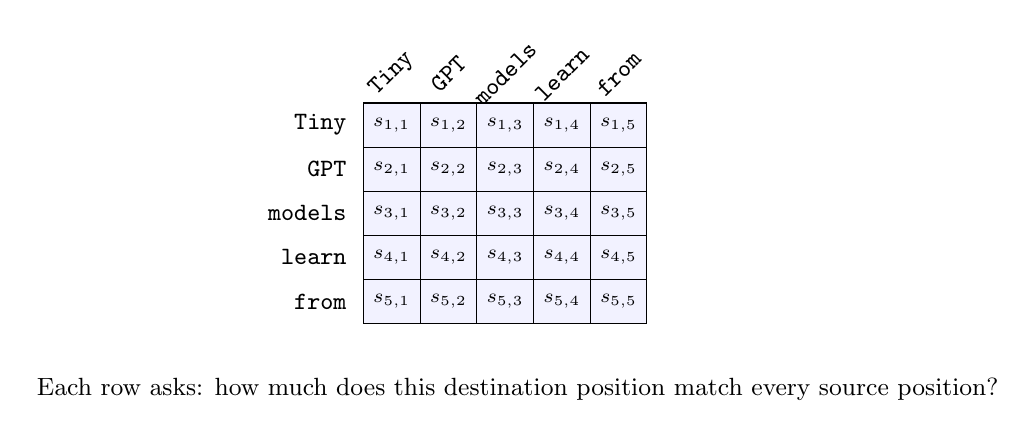
\begin{tikzpicture}[
  cell/.style={draw, minimum width=0.72cm, minimum height=0.56cm, align=center},
  note/.style={font=\small, align=center}
]
\foreach \c/\word in {0/Tiny,1/GPT,2/models,3/learn,4/from} {
  \node[note, rotate=45] at (1.4+\c*0.72,0.65) {\texttt{\word}};
  \node[note, anchor=east] at (0.95,-\c*0.56) {\texttt{\word}};
}
\foreach \r in {0,1,2,3,4} {
  \foreach \c in {0,1,2,3,4} {
    \node[cell, fill=blue!5] at (1.4+\c*0.72,-\r*0.56) {\scriptsize \(s_{\the\numexpr\r+1\relax,\the\numexpr\c+1\relax}\)};
  }
}
\node[note] at (3.0,-3.35) {Each row asks: how much does this destination position match every source position?};
\end{tikzpicture}}
\end{center}

For GPT, not every score is allowed. A position cannot read the future.

\section{The Causal Mask}

GPT is trained for next-token prediction. When predicting at position \(i\), the model must not read tokens at positions \(j>i\). The causal mask sets future scores to a very negative number before softmax:

\[
s_{i,j} =
\begin{cases}
\dfrac{q_i\cdot k_j}{\sqrt d}, & j\leq i,\\
-\infty, & j>i.
\end{cases}
\]

\begin{center}
\resizebox{0.82\textwidth}{!}{
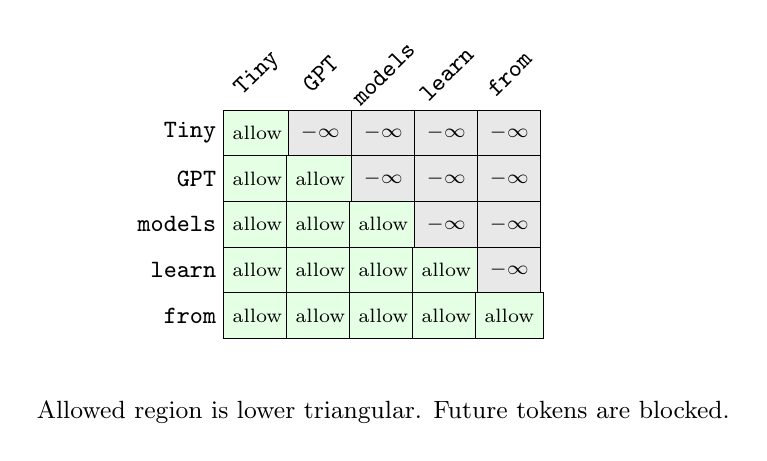
\begin{tikzpicture}[
  cell/.style={draw, minimum width=0.8cm, minimum height=0.58cm, align=center},
  note/.style={font=\small, align=center}
]
\foreach \c/\word in {0/Tiny,1/GPT,2/models,3/learn,4/from} {
  \node[note, rotate=45] at (1.4+\c*0.8,0.75) {\texttt{\word}};
  \node[note, anchor=east] at (1.0,-\c*0.58) {\texttt{\word}};
}
\foreach \r in {0,1,2,3,4} {
  \foreach \c in {0,1,2,3,4} {
    \ifnum\c>\r
      \node[cell, fill=gray!18] at (1.4+\c*0.8,-\r*0.58) {\scriptsize \(-\infty\)};
    \else
      \node[cell, fill=green!10] at (1.4+\c*0.8,-\r*0.58) {\scriptsize allow};
    \fi
  }
}
\node[note] at (3.0,-3.55) {Allowed region is lower triangular. Future tokens are blocked.};
\end{tikzpicture}}
\end{center}

Row 5 can attend to positions 1 through 5. Row 2 can attend only to positions 1 and 2. This is what prevents training from cheating.

\section{Softmax Turns Scores Into Weights}

Scores can be negative, positive, large, or small. Attention weights must be probabilities:

\[
\alpha_{i,j}\geq 0,\qquad \sum_{j\leq i}\alpha_{i,j}=1.
\]

Softmax converts the allowed scores in a row into probabilities:

\[
\alpha_{i,j}=
\frac{\exp(s_{i,j})}{\sum_{m\leq i}\exp(s_{i,m})}.
\]

For row 5 in TinyGPT, suppose the masked scores are:

\[
\begin{bmatrix}
0.2 & 0.5 & 0.1 & 0.7 & 1.0
\end{bmatrix}.
\]

Softmax might produce approximately:

\[
\begin{bmatrix}
0.13 & 0.17 & 0.12 & 0.21 & 0.27
\end{bmatrix}.
\]

\begin{center}
\begin{tikzpicture}[
  cell/.style={draw, minimum width=0.7cm, minimum height=0.5cm, align=center},
  arrow/.style={-{Latex[length=2mm]}, thick},
  note/.style={font=\small, align=center}
]
\foreach \i/\v in {0/0.2,1/0.5,2/0.1,3/0.7,4/1.0} {
  \node[cell, fill=blue!5] at (\i*0.75,0) {\scriptsize \v};
}
\node[note] at (1.5,0.65) {masked score row};
\node[draw, rounded corners=2pt, fill=yellow!18, minimum width=1.8cm, minimum height=0.65cm, align=center] (soft) at (5.0,0) {softmax};
\foreach \i/\v in {0/0.13,1/0.17,2/0.12,3/0.21,4/0.27} {
  \node[cell, fill=red!8] at (6.55+\i*0.75,0) {\scriptsize \v};
}
\node[note] at (8.0,0.65) {attention weights sum to 1};
\draw[arrow] (3.85,0) -- (soft);
\draw[arrow] (soft) -- (6.1,0);
\end{tikzpicture}
\end{center}

\section{Context Vectors}

The attention weights are applied to value vectors:

\[
z^{(i)}=\sum_{j\leq i}\alpha_{i,j}v^{(j)}.
\]

For all positions at once:

\[
Z=AV,
\]

where \(A\in\mathbb{R}^{T\times T}\) is the attention-weight matrix and \(V\in\mathbb{R}^{T\times d}\) is the value matrix.

\begin{center}
\resizebox{\textwidth}{!}{
\begin{tikzpicture}[
  cell/.style={draw, minimum width=0.58cm, minimum height=0.48cm, align=center},
  arrow/.style={-{Latex[length=2mm]}, thick},
  note/.style={font=\small, align=center}
]
\node[note] at (1.4,0.75) {attention weights \(A\)};
\foreach \r in {0,1,2,3,4} {
  \foreach \c in {0,1,2,3,4} {
    \ifnum\c>\r
      \node[cell, fill=gray!18] at (\c*0.58,-\r*0.48) {\scriptsize 0};
    \else
      \node[cell, fill=yellow!18] at (\c*0.58,-\r*0.48) {};
    \fi
  }
}
\node[note] at (4.5,0.75) {values \(V\)};
\foreach \r in {0,1,2,3,4} {
  \foreach \c in {0,1} {
    \node[cell, fill=blue!5] at (4.0+\c*0.58,-\r*0.48) {};
  }
}
\node[note] at (6.4,-1.0) {\(\times\)};
\node[note] at (8.3,0.75) {context vectors \(Z\)};
\foreach \r in {0,1,2,3,4} {
  \foreach \c in {0,1} {
    \node[cell, fill=red!8] at (7.8+\c*0.58,-\r*0.48) {};
  }
}
\draw[arrow] (5.4,-1.0) -- (7.2,-1.0);
\node[note] at (4.4,-3.1) {Every output row is a weighted mixture of value rows allowed by the causal mask.};
\end{tikzpicture}}
\end{center}

\section{The Full Single-Head Formula}

Putting the pieces together:

\[
Q=XW_Q,\qquad K=XW_K,\qquad V=XW_V,
\]

\[
S=\frac{QK^\top}{\sqrt d},
\]

\[
A=\operatorname{softmax}(\operatorname{mask}(S)),
\]

\[
Z=AV.
\]

In compact form:

\[
\operatorname{Attention}(Q,K,V)
=
\operatorname{softmax}\left(
\operatorname{mask}\left(\frac{QK^\top}{\sqrt d}\right)
\right)V.
\]

\begin{center}
\resizebox{\textwidth}{!}{
\begin{tikzpicture}[
  box/.style={draw, rounded corners=2pt, minimum height=0.65cm, text width=1.9cm, align=center},
  arrow/.style={-{Latex[length=2mm]}, thick}
]
\node[box, fill=blue!5] (x) at (0,0) {\(X\)};
\node[box, fill=yellow!18] (qkv) at (2.3,0) {linear\\Q,K,V};
\node[box, fill=red!8] (scores) at (4.6,0) {\(QK^\top/\sqrt d\)};
\node[box, fill=gray!12] (mask) at (6.9,0) {causal\\mask};
\node[box, fill=green!10] (soft) at (9.2,0) {softmax\\\(A\)};
\node[box, fill=red!8] (z) at (11.5,0) {\(AV\)\\context};
\draw[arrow] (x) -- (qkv);
\draw[arrow] (qkv) -- (scores);
\draw[arrow] (scores) -- (mask);
\draw[arrow] (mask) -- (soft);
\draw[arrow] (soft) -- (z);
\draw[arrow] (qkv) .. controls (7.0,-1.3) and (9.2,-1.3) .. node[below] {\(V\)} (z);
\end{tikzpicture}}
\end{center}

\section{Multi-Head Attention}

One attention head can learn one way to read context. Multi-head attention runs several attention heads in parallel.

If the embedding dimension is \(C\) and the number of heads is \(H\), then each head has dimension:

\[
d=\frac{C}{H}.
\]

For example, if \(C=12\) and \(H=3\):

\[
d=4.
\]

The tensor shape changes like this:

\[
\shape{[B,T,C]}
\rightarrow
\shape{[B,T,H,d]}
\rightarrow
\shape{[B,H,T,d]}.
\]

\begin{center}
\resizebox{\textwidth}{!}{
\begin{tikzpicture}[
  box/.style={draw, rounded corners=2pt, minimum height=0.7cm, text width=2.35cm, align=center},
  arrow/.style={-{Latex[length=2mm]}, thick},
  note/.style={font=\small, align=center}
]
\node[box, fill=blue!5] (x) at (0,0) {hidden\\\shape{[B,T,12]}};
\node[box, fill=yellow!18] (split) at (3,0) {split channels\\3 heads};
\node[box, fill=red!8] (h0) at (6,1.1) {head 0\\\shape{[B,T,4]}};
\node[box, fill=red!8] (h1) at (6,0) {head 1\\\shape{[B,T,4]}};
\node[box, fill=red!8] (h2) at (6,-1.1) {head 2\\\shape{[B,T,4]}};
\node[box, fill=green!10] (cat) at (9.2,0) {concatenate\\\shape{[B,T,12]}};
\node[box, fill=gray!12] (proj) at (12.1,0) {output\\projection};
\draw[arrow] (x) -- (split);
\draw[arrow] (split) -- (h0);
\draw[arrow] (split) -- (h1);
\draw[arrow] (split) -- (h2);
\draw[arrow] (h0) -- (cat);
\draw[arrow] (h1) -- (cat);
\draw[arrow] (h2) -- (cat);
\draw[arrow] (cat) -- (proj);
\node[note] at (6,-2.0) {Different heads can learn different reading patterns.};
\end{tikzpicture}}
\end{center}

The heads might specialize loosely:

\begin{itemize}
  \item one head may track local grammar;
  \item one head may copy a recent noun;
  \item one head may identify punctuation or boundaries.
\end{itemize}

These descriptions are intuition, not guaranteed labels. Heads are learned by the loss, not assigned by a human.

\section{Multi-Head Shape Trace}

For \(B=2\), \(T=4\), \(C=12\), and \(H=3\):

\begin{lstlisting}
x:                   [2, 4, 12]
qkv projection:       [2, 4, 36]     # 3*C
split q, k, v:        [2, 4, 12] each
reshape heads:        [2, 4, 3, 4]
transpose:            [2, 3, 4, 4]
attention scores:     [2, 3, 4, 4]
attention weights:    [2, 3, 4, 4]
head outputs:         [2, 3, 4, 4]
transpose back:       [2, 4, 3, 4]
concatenate:          [2, 4, 12]
output projection:    [2, 4, 12]
\end{lstlisting}

This shape trace is one of the best ways to debug attention code.

\section{Causal Self-Attention Source Code}

A compact PyTorch attention module can compute \(Q,K,V\) with one linear layer:

\begin{lstlisting}[language=Python]
class CausalSelfAttention(nn.Module):
    def __init__(self, config):
        super().__init__()
        assert config.n_embd % config.n_head == 0
        self.n_head = config.n_head
        self.n_embd = config.n_embd
        self.head_dim = config.n_embd // config.n_head

        self.c_attn = nn.Linear(config.n_embd, 3 * config.n_embd)
        self.c_proj = nn.Linear(config.n_embd, config.n_embd)
        self.dropout = nn.Dropout(config.dropout)

        mask = torch.tril(torch.ones(config.block_size, config.block_size))
        self.register_buffer("mask", mask.view(1, 1, config.block_size, config.block_size))

    def forward(self, x):
        B, T, C = x.shape
        q, k, v = self.c_attn(x).split(C, dim=2)   # each [B, T, C]

        q = q.view(B, T, self.n_head, self.head_dim).transpose(1, 2)
        k = k.view(B, T, self.n_head, self.head_dim).transpose(1, 2)
        v = v.view(B, T, self.n_head, self.head_dim).transpose(1, 2)
        # q, k, v: [B, H, T, d]

        scores = (q @ k.transpose(-2, -1)) / math.sqrt(self.head_dim)
        scores = scores.masked_fill(self.mask[:, :, :T, :T] == 0, float("-inf"))
        weights = torch.softmax(scores, dim=-1)
        weights = self.dropout(weights)

        y = weights @ v                           # [B, H, T, d]
        y = y.transpose(1, 2).contiguous().view(B, T, C)
        return self.c_proj(y)                     # [B, T, C]
\end{lstlisting}

Important details:

\begin{itemize}
  \item \texttt{register\_buffer} stores the mask with the model but does not train it;
  \item \texttt{dim=-1} softmax means probabilities sum across source positions;
  \item \texttt{masked\_fill} blocks future positions before softmax;
  \item \texttt{contiguous()} makes memory layout safe before \texttt{view};
  \item the output shape matches the input shape \shape{[B,T,C]}.
\end{itemize}

\section{The Transformer Block}

A GPT block combines:

\begin{itemize}
  \item LayerNorm;
  \item causal self-attention;
  \item residual connection;
  \item LayerNorm;
  \item MLP;
  \item residual connection.
\end{itemize}

In pre-norm form:

\[
X' = X + \operatorname{Attention}(\operatorname{LN}_1(X)),
\]

\[
Y = X' + \operatorname{MLP}(\operatorname{LN}_2(X')).
\]

\begin{center}
\resizebox{\textwidth}{!}{
\begin{tikzpicture}[
  box/.style={draw, rounded corners=2pt, minimum height=0.62cm, text width=1.7cm, align=center},
  arrow/.style={-{Latex[length=2mm]}, thick},
  plus/.style={circle, draw, minimum size=0.5cm, align=center}
]
\node[box, fill=blue!5] (x) at (0,0) {\(X\)};
\node[box, fill=yellow!18] (ln1) at (2,0) {LN};
\node[box, fill=red!8] (attn) at (4,0) {causal\\attention};
\node[plus] (add1) at (6,0) {\(+\)};
\node[box, fill=blue!5] (xp) at (7.5,0) {\(X'\)};
\node[box, fill=yellow!18] (ln2) at (9.5,0) {LN};
\node[box, fill=red!8] (mlp) at (11.5,0) {MLP};
\node[plus] (add2) at (13.5,0) {\(+\)};
\node[box, fill=green!10] (y) at (15,0) {\(Y\)};
\draw[arrow] (x) -- (ln1);
\draw[arrow] (ln1) -- (attn);
\draw[arrow] (attn) -- (add1);
\draw[arrow] (add1) -- (xp);
\draw[arrow] (x) .. controls (2,-1.1) and (4,-1.1) .. (add1);
\draw[arrow] (xp) -- (ln2);
\draw[arrow] (ln2) -- (mlp);
\draw[arrow] (mlp) -- (add2);
\draw[arrow] (add2) -- (y);
\draw[arrow] (xp) .. controls (9.5,-1.1) and (11.5,-1.1) .. (add2);
\end{tikzpicture}}
\end{center}

Attention mixes information across positions. The MLP transforms the feature vector at each position independently.

\section{The MLP}

The Transformer MLP is a small neural network applied to each position:

\[
\operatorname{MLP}(x)=W_2\phi(W_1x+b_1)+b_2.
\]

A common GPT choice expands the channel dimension by a factor of four:

\[
C\rightarrow 4C\rightarrow C.
\]

\begin{center}
\begin{tikzpicture}[
  box/.style={draw, rounded corners=2pt, minimum height=0.65cm, text width=2.05cm, align=center},
  arrow/.style={-{Latex[length=2mm]}, thick},
  note/.style={font=\small, align=center}
]
\node[box, fill=blue!5] (in) at (0,0) {one position\\\shape{[C]}};
\node[box, fill=red!8] (up) at (2.7,0) {linear\\\shape{[4C]}};
\node[box, fill=yellow!18] (gelu) at (5.4,0) {GELU\\nonlinearity};
\node[box, fill=red!8] (down) at (8.1,0) {linear\\\shape{[C]}};
\node[box, fill=green!10] (out) at (10.8,0) {updated\\features};
\draw[arrow] (in) -- (up);
\draw[arrow] (up) -- (gelu);
\draw[arrow] (gelu) -- (down);
\draw[arrow] (down) -- (out);
\node[note] at (5.4,-0.9) {Same MLP weights are reused at every token position.};
\end{tikzpicture}
\end{center}

Why have both attention and MLP?

\begin{itemize}
  \item attention lets positions exchange information;
  \item the MLP computes richer features at each position after exchange;
  \item residual connections preserve the old state while adding new information.
\end{itemize}

\section{Transformer Block Source Code}

A minimal GPT block:

\begin{lstlisting}[language=Python]
class Block(nn.Module):
    def __init__(self, config):
        super().__init__()
        self.ln_1 = nn.LayerNorm(config.n_embd)
        self.attn = CausalSelfAttention(config)
        self.ln_2 = nn.LayerNorm(config.n_embd)
        self.mlp = nn.Sequential(
            nn.Linear(config.n_embd, 4 * config.n_embd),
            nn.GELU(),
            nn.Linear(4 * config.n_embd, config.n_embd),
            nn.Dropout(config.dropout),
        )

    def forward(self, x):
        x = x + self.attn(self.ln_1(x))
        x = x + self.mlp(self.ln_2(x))
        return x
\end{lstlisting}

The code is short because each object has a clear contract:

\begin{longtable}{p{0.24\textwidth}p{0.22\textwidth}p{0.38\textwidth}}
\toprule
\term{Line part} & \term{Shape} & \term{Meaning} \\
\midrule
\texttt{ln\_1(x)} & \shape{[B,T,C]} & stabilize features before attention \\
\texttt{attn(...)} & \shape{[B,T,C]} & mix information across positions \\
\texttt{x + ...} & \shape{[B,T,C]} & residual update \\
\texttt{ln\_2(x)} & \shape{[B,T,C]} & stabilize features before MLP \\
\texttt{mlp(...)} & \shape{[B,T,C]} & transform features at each position \\
\bottomrule
\end{longtable}

\section{Attention Versus MLP: Who Does What}

\begin{center}
\resizebox{0.95\textwidth}{!}{
\begin{tikzpicture}[
  box/.style={draw, rounded corners=2pt, minimum height=0.65cm, text width=2.7cm, align=center},
  arrow/.style={-{Latex[length=2mm]}, thick},
  note/.style={font=\small, align=center}
]
\node[box, fill=blue!5] (tokens) at (0,0) {positions\\\texttt{Tiny GPT models learn}};
\node[box, fill=red!8] (attn) at (4,0.8) {attention\\mixes across positions};
\node[box, fill=yellow!18] (mlp) at (4,-0.8) {MLP\\transforms features};
\node[box, fill=green!10] (out) at (8,0) {better hidden states\\for prediction};
\draw[arrow] (tokens) -- (attn);
\draw[arrow] (tokens) -- (mlp);
\draw[arrow] (attn) -- (out);
\draw[arrow] (mlp) -- (out);
\node[note] at (4,-1.75) {Attention asks where to read. MLP asks what features to compute after reading.};
\end{tikzpicture}}
\end{center}

\section{Engineering Practice}

Attention implementations should test:

\begin{itemize}
  \item no position attends to future tokens;
  \item attention weights sum to one over allowed source positions;
  \item \(C\) is divisible by \(H\);
  \item output shape matches input shape;
  \item the causal mask slices correctly for shorter sequences;
  \item dropout is active only during training;
  \item CPU and GPU results have matching shapes and similar loss behavior.
\end{itemize}

For a teaching repo, keep at least one debug mode that returns attention weights. Do not use that mode during high-performance training by default, but it is extremely helpful for learning and tests.

\section{Hands-On Lab: Build And Inspect Causal Attention}

Create a small script with \(B=1\), \(T=5\), \(C=12\), and \(H=3\). Build random hidden states:

\begin{lstlisting}[language=Python]
import math
import torch
import torch.nn.functional as F

torch.manual_seed(3)
B, T, C, H = 1, 5, 12, 3
d = C // H
x = torch.randn(B, T, C)

qkv = torch.nn.Linear(C, 3*C, bias=False)
q, k, v = qkv(x).split(C, dim=2)

q = q.view(B, T, H, d).transpose(1, 2)
k = k.view(B, T, H, d).transpose(1, 2)
v = v.view(B, T, H, d).transpose(1, 2)

scores = (q @ k.transpose(-2, -1)) / math.sqrt(d)
mask = torch.tril(torch.ones(T, T)).view(1, 1, T, T)
scores = scores.masked_fill(mask == 0, float("-inf"))
weights = F.softmax(scores, dim=-1)
y = weights @ v

print("q:", q.shape)
print("scores:", scores.shape)
print("weights row 4:", weights[0, 0, 4])
print("future weight from row 2 to col 4:", weights[0, 0, 2, 4])
print("y:", y.shape)
\end{lstlisting}

Expected facts:

\begin{itemize}
  \item \texttt{q} has shape \shape{[1,3,5,4]};
  \item \texttt{scores} has shape \shape{[1,3,5,5]};
  \item future weights are zero after softmax;
  \item \texttt{y} has shape \shape{[1,3,5,4]} before heads are concatenated.
\end{itemize}

\checkpoint

\begin{enumerate}
  \item What problem does attention solve in TinyGPT?
  \item What are queries, keys, and values?
  \item Why is the score \(q_i\cdot k_j\) divided by \(\sqrt d\)?
  \item Why does GPT use a causal mask?
  \item What does softmax do to each score row?
  \item Why does multi-head attention split \(C\) into \(H\) heads?
  \item What shape are attention scores for \(B=2\), \(H=3\), and \(T=4\)?
  \item In a Transformer block, what is the difference between attention and the MLP?
\end{enumerate}

\subsection*{Solutions}

\begin{enumerate}
  \item Attention lets each token position read useful information from earlier positions, so prediction is based on context rather than only the current token vector.
  \item A query describes what a destination position is looking for, a key describes what a source position offers for matching, and a value contains the information copied into the context vector.
  \item The scaling keeps dot-product magnitudes stable as the head dimension grows, preventing softmax from becoming too sharp too early.
  \item GPT predicts next tokens left to right. If a position could read future tokens during training, it would cheat and fail to learn the real generation task.
  \item Softmax converts allowed scores into nonnegative probabilities that sum to one across source positions.
  \item Multiple heads let the model learn several attention patterns in parallel, each in a lower-dimensional subspace.
  \item The score tensor has shape \shape{[2,3,4,4]}: batch, head, destination position, source position.
  \item Attention mixes information across token positions. The MLP transforms the feature vector at each position independently after attention has mixed context.
\end{enumerate}
